\documentclass[UTF8]{ctexart}
% \usepackage{amsfonts}
% \usepackage{amsmath}
% \usepackage{amssymb}
% \usepackage{amsthm}
% \usepackage{booktabs}
\usepackage{courier}
% \usepackage{float}
\usepackage{geometry}
\usepackage{graphicx}
% \usepackage{hyperref}
% \usepackage{listings}
\geometry{left=2.54cm,right=2.54cm,top=2.18cm,bottom=3.18cm}

\begin{document}

\title{人脸表情识别——中期报告}
\author{无46\ \ 严靖凯\ \ 2014011192\\ 无46\ \ 王启睿\ \ 2014011179\\ 无46\ \ 黄秀峰\ \ 2014011193}
\maketitle

\section{概述}

% 最好在里面加一些参考文献吧。
% 还要加点什么你们看吧~

对于人脸表情识别问题,目前学术界已有了较为充分的研究。对该问题的处理方法,大体可分为传统模式识别和神经网络两类。其中,传统模式识别方式的代表性文章有\cite{happy2015automatic,islam2016sention,wang2013feature,salmam2016facial}等,其中大多数采用SVM或决策树进行判决,神经网络方式的代表性文章有\cite{BarsoumICMI2016,khorrami2015deep}等。传统方法往往训练和运行速度很快,部分方法甚至可以应用于实时视频流作为输入等场景,对于质量高(清晰、光照合适、正脸)的图片也有很高的识别正确率;而神经网络方法对于一些传统方法难以完成的情形如很低的图片分辨率、不理想的光照、侧脸,或视频片段等。

由于本课程实验给了比较充裕的时间,因此我们考虑对这两种方法都进行一下尝试,一方面是为了验证究竟哪种特征提取与识别方法能获得更好的效果,另一方面也是为了对这些方法都进行练习,以熟悉其方法与技能。

目前,我们着重考虑了两种方法,分别属于神经网络和传统模式时变的范畴,以下将对它们进行详细介绍。

\section{方法一:CNN(VGG-13)网络特征提取}

我们本次实验提供的数据集上的数据量相对较小,而神经网络方法需要较大的训练集作为支撑,\cite{BarsoumICMI2016}提供的FER+数据集中有较多数据,因此我们选择%原谅她啊
在FER+数据集上复现文\cite{BarsoumICMI2016}的效果。

\begin{figure}[ht]
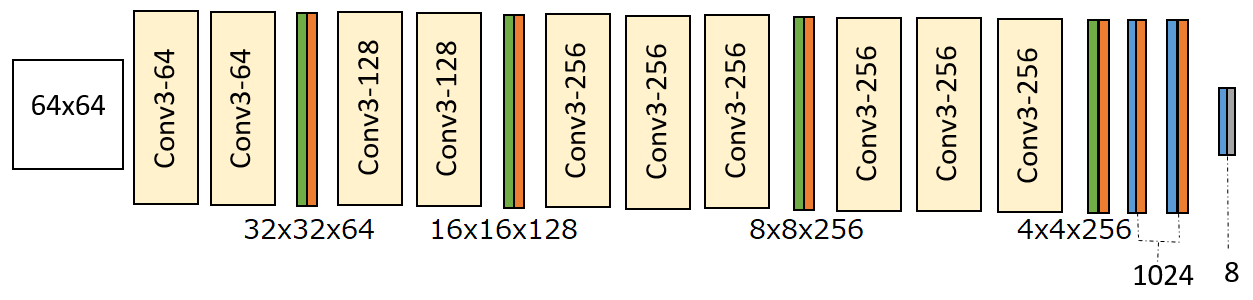
\includegraphics[width=\textwidth]{ferplus.png}
\caption{测试使用的CNN结构}\label{fig:ferplus}
\end{figure}

整个网络结构如上图所示,输入为为64x64灰度图片,其后的黄、绿、橙、蓝、灰色分别对应于卷积层、最大池化层、Dropout层、全连接+ ReLU层、Softmax层。该网络自VGG-13修改而来,以适应低分辨率的FER数据集。

训练得到的准确率在85\% 左右,与文中得到的结果基本一致。

事实上,该准确率很大程度上是受FER+数据集自身所限。FER数据集使用48x48的8bit灰度图片,且包含各种姿势(如侧脸、捂脸等),相比本次实验中最终需要测试的CK+、JAFFE等高分辨率正脸数据集而言,识别难度难度更大。针对前述测试数据集,下文提到的传统方法能够在更短时间、更小训练集下取得相仿甚至更高的正确率。

\section{方法二:HOG特征+SVM分类}

% 把从头到尾的理论写一下吧
% 然后就说具体的HOG特征提取代码还有待完善,还没有能整合起来测试

% 我们已经学习了libSVM的使用,并对libSVM自身的多类分类输出,针对我们的问题进行了改进,使得可以输出样本属于每一类的概率。

\section{进一步的工作}

CNN方面,我们考虑将网络换回VGG的224x224x3输入分辨率,或使用预训练好的VGG作为前级,以减小图片降采样和灰度化带来的信息损失,从而可能获得更高的正确率。

% 这一块和下一块就麻烦您二位写一下了……

\section{实验心得与体会}

% 本次实验中通过阅读文献对CNN有了更加直观的理解,同时学会了使用或调整现有的结构和成果以实现特定的功能。

% 中期报告真的需要这部分么

\bibliographystyle{unsrt}
\bibliography{midref}

\end{document}
